\documentclass[12pt,a4paper,oneside,openany]{memoir}

\usepackage[utf8]{inputenc}
\usepackage[frenchb]{babel}
\usepackage[T1]{fontenc}

% Paquets utiles
\usepackage{graphicx}
\usepackage[usenames,svgnames]{xcolor}
\usepackage{tikz}
\usepackage{asymptote}
\usepackage{flafter}
\usepackage{multirow}
\usepackage{ifdraft}
\usepackage{units}
\usepackage{booktabs}
\usepackage{biblatex}
\bibliography{master}
%\usepackage[pdfpagelabels,draft,implicit=false]{hyperref}

%Tkiz
\usetikzlibrary{calc}
\usetikzlibrary{arrows}


% Décoration
\usepackage[lighttt]{lmodern} % pour le tt


% POUR MATHDESIGN : restaurer hrulefill
\let\xhrf\hrulefill
\usepackage[utopia]{mathdesign}
\let\hrulefill\xhrf
\renewcommand*{\chapterheadstart}{\begingroup
	\vspace*{\beforechapskip}%
	\begin{adjustwidth}{}{-\chapindent}%
		\hrulefill
		\smash{\rule{0.4pt}{15mm}}
	\end{adjustwidth}\endgroup}
%\usepackage{tgpagella}
\let\mathbb\relax \usepackage{bbold}
\fixpdflayout
%\counterwithout{section}{chapter}
%\setsecnumdepth{subsection}


\chapterstyle{ell}
\setsecheadstyle{\Large\bfseries\sffamily\raggedright}
\setsubsecheadstyle{\large\bfseries\sffamily\raggedright}
\midsloppy

\makepagestyle{myruled}
\makeoddfoot{myruled}{}{\thepage}{}
\makeevenfoot{myruled}{}{\thepage}{}
\makeheadrule{myruled}{\textwidth}{\normalrulethickness}
\makeevenhead{myruled}{\rightmark}{}{}
\makeoddhead{myruled}{\rightmark}{}{}
\pagestyle{myruled}

\captiondelim{ : }
\captiontitlefont{\sffamily}

\newsubfloat{figure}
\newsubfloat{table}

\newcommand{\anonchapter}[1]{\chapter*{#1}\addcontentsline{toc}{chapter}{\numberline{}#1}}
\newcommand{\todo}[1]{\marginpar{\textcolor{red}{#1}}}
\newcommand{\fltbrule}{\hrule\vspace{\onelineskip}}
\newcommand{\fltarule}{\vspace{\onelineskip}
	\hrule\vspace{\onelineskip}}

\author{Charles Bine\\Matthieu Félix}
\title{\\Production d'énergie électrique (centrales nucléaires et barrages hydroélectriques)}
\date{Décembre 2015}


% EXEMPLES & référence rapide
% dessin asymptote
% \lstinputlisting[firstline=, lastline=]{fichier}

\begin{document}
	
% Page de titre
\keepthetitle
\begin{titlingpage}
\noindent
\begin{minipage}[t]{0.5\textwidth} \begin{flushleft}
\theauthor \\ \thedate
\end{flushleft} \end{minipage}
\begin{minipage}[t]{0.5\textwidth} \begin{flushright}
Rapport de projet \\
Cours de réseaux électriques
\end{flushright} \end{minipage}

\vspace{3cm}
\begin{center}
{\LARGE \textbf{\thetitle}}
\ifdraft{\par Brouillon}{}
\end{center}
\vspace{3cm}

\end{titlingpage}

\addtolength{\marginparwidth}{11mm}
\abnormalparskip{4mm}

\clearpage

\tableofcontents
\listoffigures
\listoftables
\clearpage


\chapter{Introduction}

Dans le sillage de la mondialisation, les enjeux de la production et de la consommation énergétiques sont capitaux. La demande énergétique mondiale, toujours croissante, requiert l'inauguration d'un nombre toujours plus important de centrales de production d'énergie.

Mais comment produire durablement cette énergie? Quelles méthodes choisir? Comment respecter aux mieux les recommandation établies lord de la COP 21 à Paris? 


\chapter{Aperçu de la production d'énergie électrique}

Les principales ressources énergétiques sont les énergies fossiles (le gaz naturel, le charbon, le pétrole), l’énergie hydroélectrique, l’énergie éolienne, l’énergie nucléaire, l’énergie solaire et l'énergie géothermique. 

Étant donné les impacts environnementaux des énergies fossiles, nous nous attarderons dans cet article à l'analyse de deux types de production d'énergie électrique renouvelable: les centrales nucléaires et les barrages hydroélectriques. 

\section{Production mondiale}

L'électricité est communément présentée comme une "énergie propre". En effet les équipements l'utilisant n'émettent aucun gaz polluant ni gaz à effet de serre directement du fait de l'utilisation de l'énergie électrique.
Toutefois l'électricité n'est pas une énergie disponible naturellement sur Terre ; elle est donc produite par conversion d'autres formes d'énergie en énergie électrique.
Or la plupart des processus de production d'électricité, et en particulier ceux les plus répandus au début du XX\ieme{} siècle, ont des effets néfastes sur l'environnement :


\paragraph{Les centrales thermiques} rejettent des oxydes de soufre, d'azote et des suies et surtout émettent d'importantes quantités de CO2 (principal gaz à effet de serre) ;
\paragraph{Les centrales nucléaires} produisent des déchets radioactifs dont la durée de vie peut dépasser le millénaire ;
\paragraph{Les grands barrages hydroélectriques}  modifient profondément les écosystèmes (Voir Barrage des Trois-Gorges en Chine);
\paragraph{Les éoliennes} défigureraient, aux yeux de certains, les paysages.


L'électricité, comme toutes les formes ou vecteurs énergétiques, génère donc des impacts environnementaux, économiques et sociaux que l'on cherche à limiter. Toutefois, la répartition des formes d'énergie laisse toujours à désirer. En effet, les figures \ref{fig:monde1} et \ref{fig:monde2} montrent la prédominance des énergies fossiles dans le monde.

\begin{figure}[h]
	\centering]\hspace*{-5mm}
	\begin{minipage}{.5\textwidth}
		\centering
		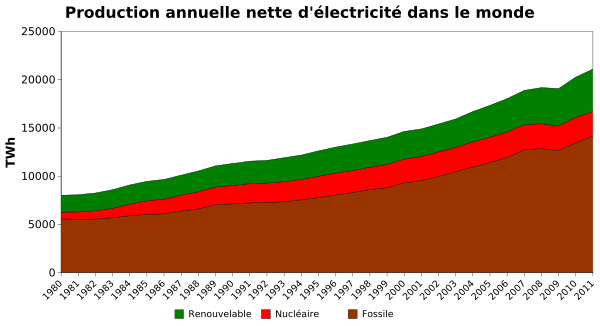
\includegraphics[width=\linewidth]{img/monde1.png}
		\caption{Évolution de la répartition de la production d'énergie mondiale}
		\label{fig:monde1}
	\end{minipage}%
	\hspace*{1cm}
	\begin{minipage}{.5\textwidth}
		\centering
		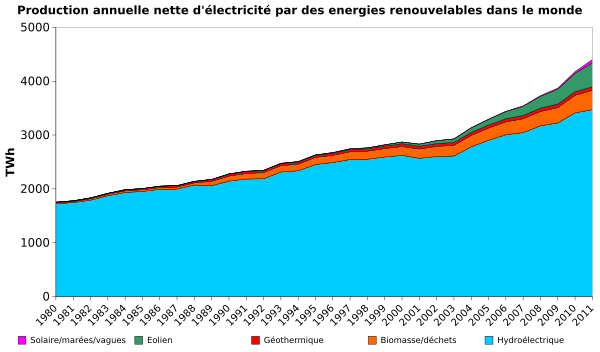
\includegraphics[width=\linewidth]{img/monde2.png}
		\caption{Évolution de la répartition de la production d'énergie renouvelable mondiale}
		\label{fig:monde2}
	\end{minipage}
\end{figure}



\section{Production Française}

Après la disparition complète de la production française de charbon en 2005, le pétrole, le gaz et surtout l’électricité sont les principales énergies consommées en France. Si la France ne produit plus de pétrole brut que de façon marginale, les treize raffineries implantées sur le territoire permettent de satisfaire plus de 90 \% de la demande nationale. Le groupe français Total, qui possède des concessions dans le monde entier, est la sixième entreprise mondiale et la cinquième du secteur. La part du gaz dans la consommation énergétique française a fortement augmenté depuis les années 1970, mais il s’agit à 97 \% de gaz importé, notamment de Russie, d’Algérie et de la mer du Nord. 

En revanche, la France produit plus d’électricité qu’elle n’en consomme, notamment grâce à 59 réacteurs nucléaires (le second parc mondial après le parc américain) qui produisaient en 2013 près de 74\% de l’électricité du pays, mais dont le bilan environnemental est l’objet de débats. Quant aux énergies renouvelables, leur part dans la production électrique française augmente et s’établit en 2013 à près de 17 \%, en grande partie grâce à l’hydroélectrique. 

Le tableau \ref{repartition production} détaille les différents composants de la production énergétique française en fonction du type de production d'énergie.

	\begin{table}[h]
		\centering
		\begin{tabular}{cc}
			\toprule
			Filière & Répartition\\
			\midrule
			Nucléaire & $74\%$ \\ 
			Hydro & $13,3\%$ \\ 
			Thermique & $7,8\%$ \\ 
			Éoliennes & $2,8\%$ \\ 
			Autres & $0,9\%$ \\ 
			Biomasse & $0,7\%$ \\ 
			\bottomrule
		\end{tabular} 
		\caption{Répartition de la production énergétique par filière}
		\label{repartition production}
	\end{table}


La consommation française d'électricité s'élève à environ \unit[480]{TWh} par an. Cependant, la consommation est assujettie à des fluctuations parfois importantes, souvent dues à des contingences météorologiques. 

\begin{figure}[h]
	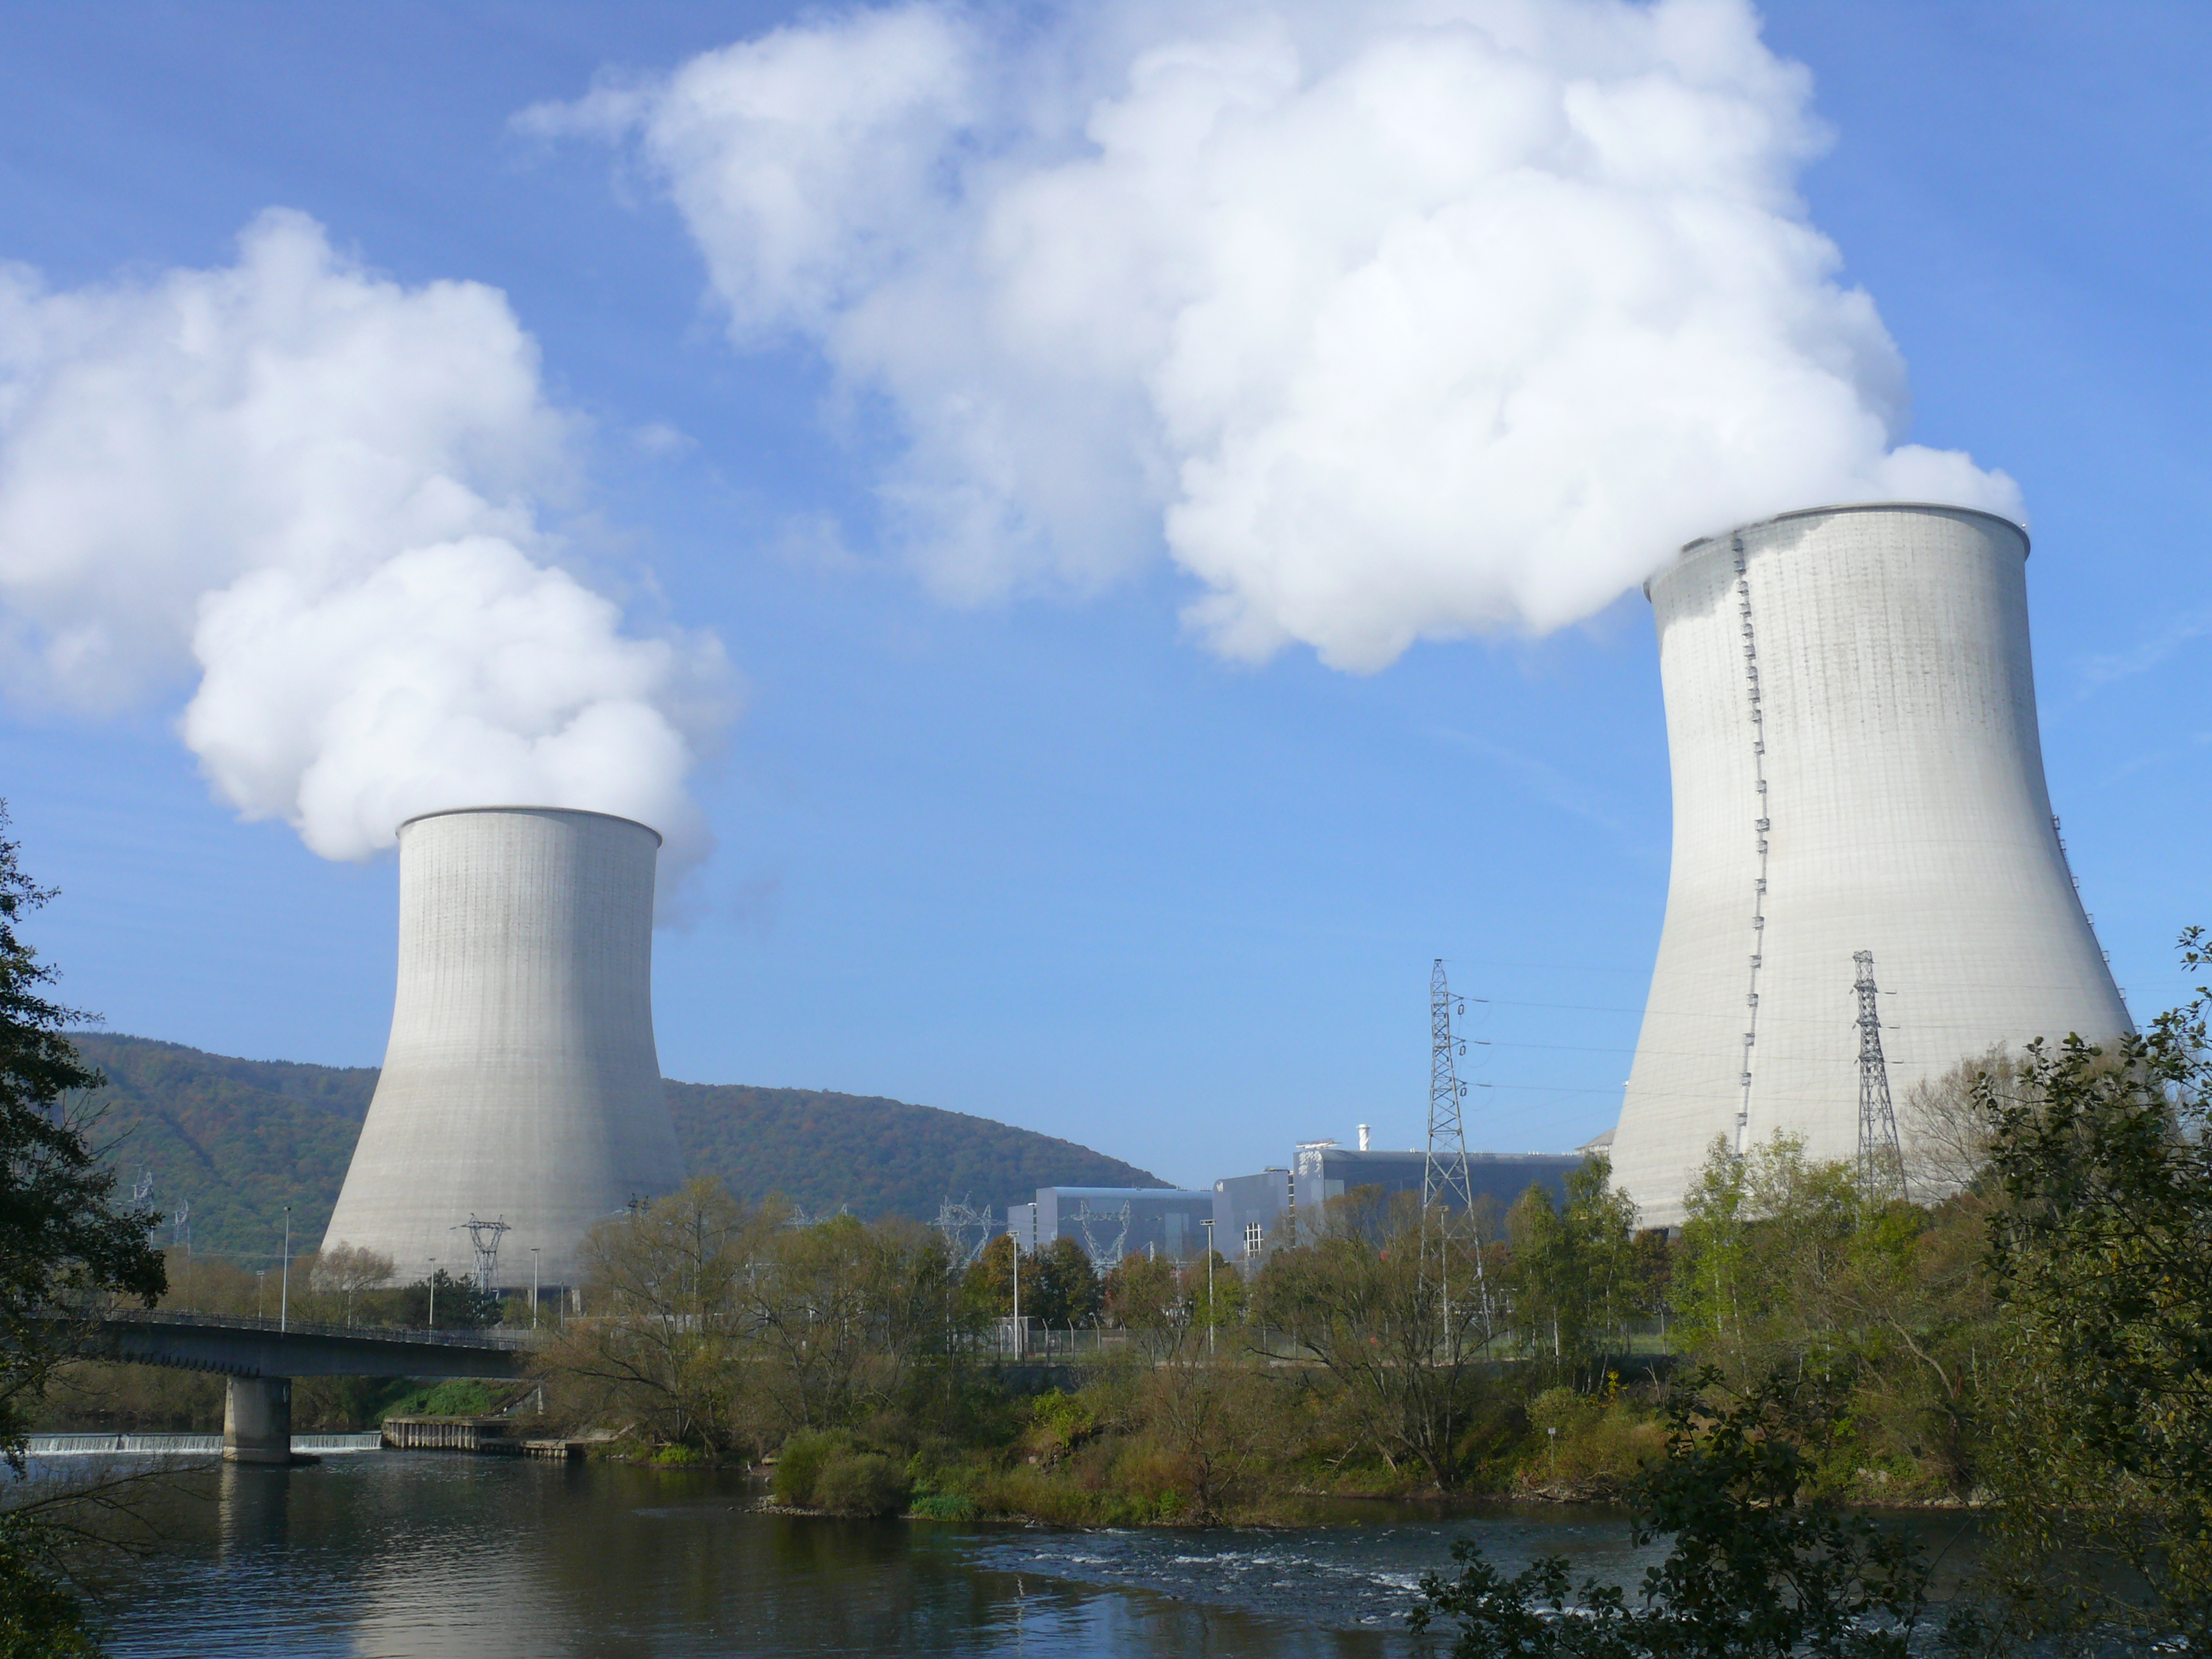
\includegraphics[width=\textwidth]{img/centrale1.jpeg}
	\caption[Une photographie de la Centrale nucléaire de Chooz]{Une photographie de la Centrale nucléaire de Chooz, construite et opérée par EDF.}
\end{figure}

La répartition de la consommation de l'électricité par secteur est représentée dans la table \ref{repartition secteur}. On constate que les deux tiers de la consommation française sont dus aux ménages et aux transports.



	\begin{table}[h]
		\centering
		\begin{tabular}{cc}
			\toprule
			Secteur & Répartition\\
			\midrule
			Ménages & $30,3\%$ \\ 
			Industrie & $19,4\%$ \\ 
			Transports & $31,1\%$ \\ 
			Services & $16\%$ \\ 
			Agriculture & $3\%$ \\ 
			Pèche & $0,2\%$ \\ 
			\bottomrule
		\end{tabular} 
		\caption{Répartition de la consommation énergétique par secteur}
		\label{repartition secteur}
	\end{table}


\chapter{Le turbo-alternateur, au cœur de la production d'énergie électrique}

\begin{figure}
	\centering
	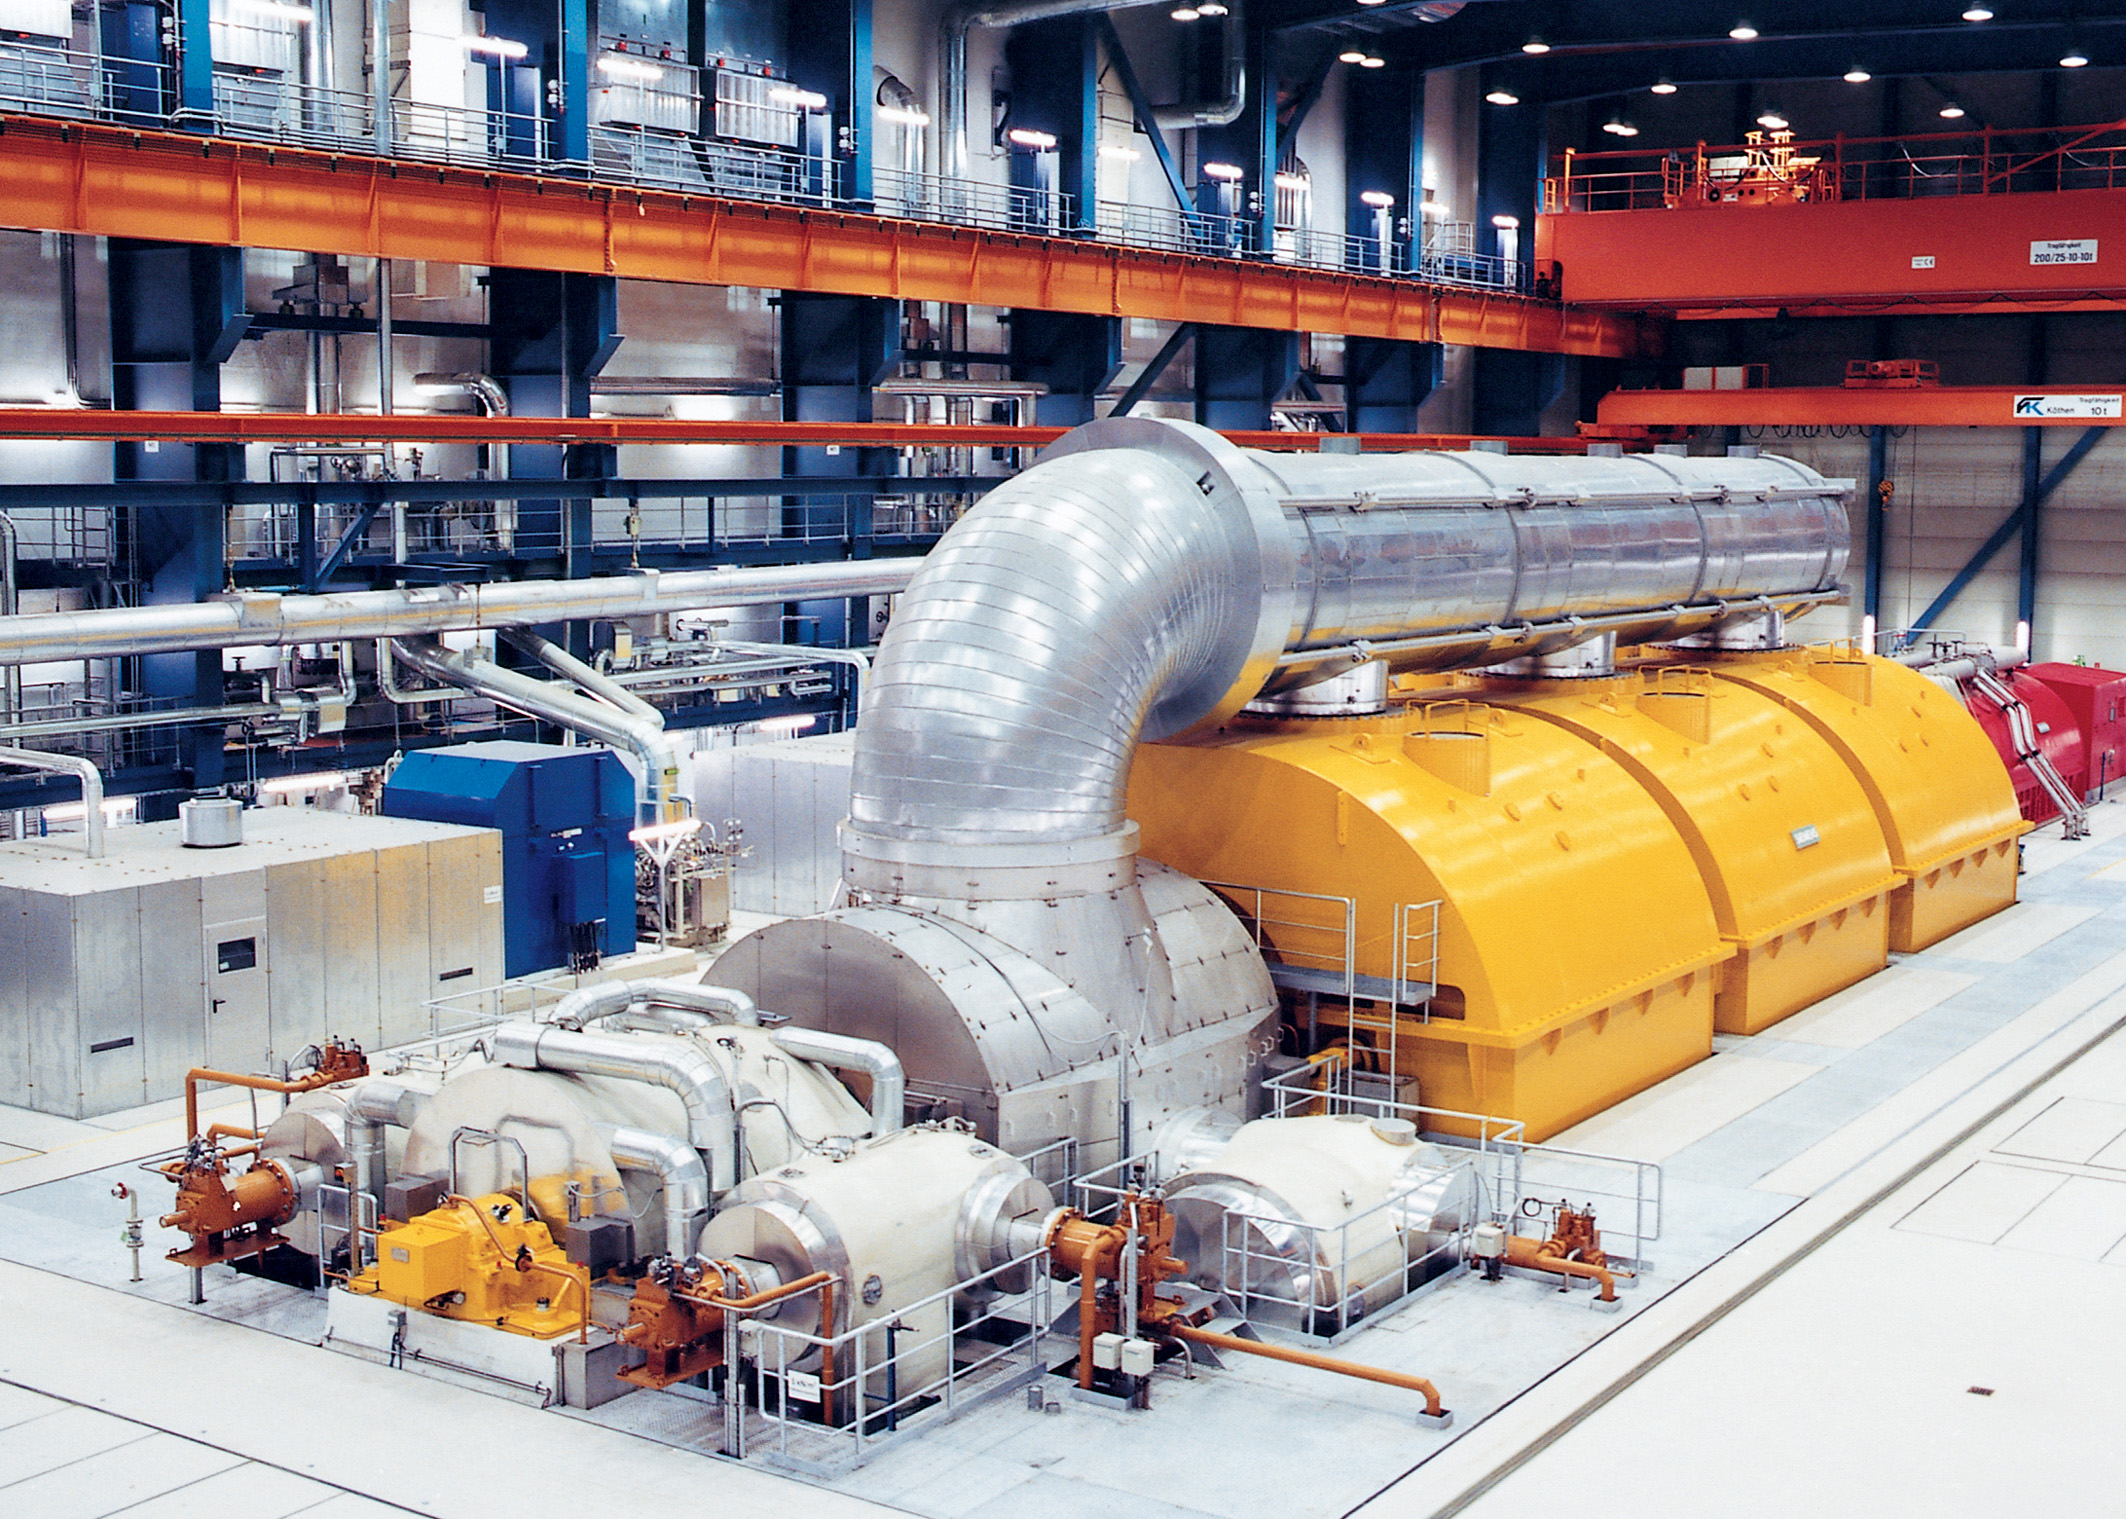
\includegraphics[width=0.95\linewidth]{img/Turbogenerator01}
	\caption{Un turbo-alternateur moderne}
	\label{fig:turbogenerator}
\end{figure}

\begin{figure}
	\centering
	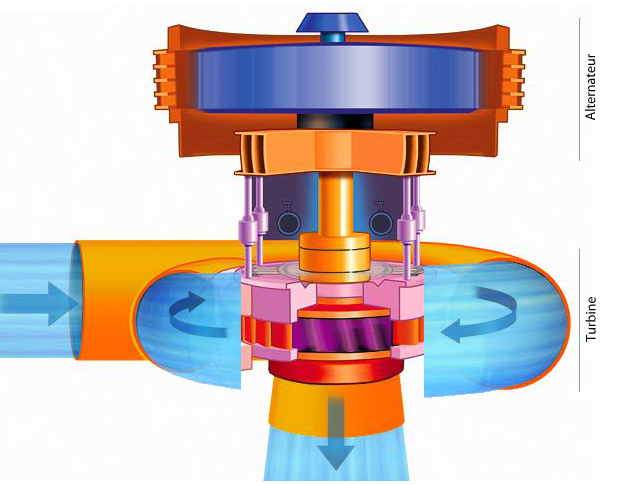
\includegraphics[width=0.9\linewidth]{img/coupe_turbo_alternateur}
	\caption{Un turbo-alternateur à eau vu en coupe}
	\label{fig:coupe_turbo_alternateur}
\end{figure}

De nombreux types de centrales modernes (à gaz, à charbon, hydro-électriques, nucléaires,\textellipsis) fonctionnent à l'aide de \emph{turbo-alternateurs} : une association entre une turbine et un alternateur.

\section{Turbine}
Afin de produire la force mécanique nécessaire, le fluide (eau ou gaz) passe par une turbine. Les turbines à gaz ont un axe parallèle au sens de déplacement du fluide, et sont composées d'hélices successives qui captent l'énergie cinétique du gaz.

Dans le cas des turbines à eau, l'eau est conduite dans un mouvement circulaire autour de l'hélice de la turbine.

\section{Alternateur}
L'alternateur permet de convertir un mouvement mécanique de rotation, fourni par la turbine, en un courant électrique alternatif généralement triphasé.

L'alternateur fonctionne avec un rotor et un stator. Le rotor est entraîné par la turbine et est composé d'une série d'électroaimants ; le stator est fixé au bâti, et est recouvert de bobines dans lesquelles le courant sera induit.

Le bobinage de cette partie s'effectue comme celui des machines à courant alternatif, décrit dans le cours. On notera qu'il est assez fréquent que le bobinage du stator soit fait avec plus de deux pôles, ce qui permet de réduire la vitesse de rotation en conservant la fréquence du courant produit. Ainsi, les grandes centrales hydroélectriques utilisent généralement entre 16 et 64 pôles dans leurs alternateurs.

Le fait que les électroaimants soient situés sur le rotor pose également un problème, puisqu'ils doivent être alimentés. Plutôt que d'utiliser des balais et une piste circulaire pour transmettre le courant, les grands turbo-alternateurs se composent en fait de deux alternateurs. L'alternateur secondaire est monté dans la configuration inverse, c'est à dire que les aimants sont montés sur le stator et le bobinage passif est monté sur le rotor. Le courant ainsi produit sur le rotor est redressé, puis utilisé pour alimenter les électroaimants.

\begin{figure}
\centering
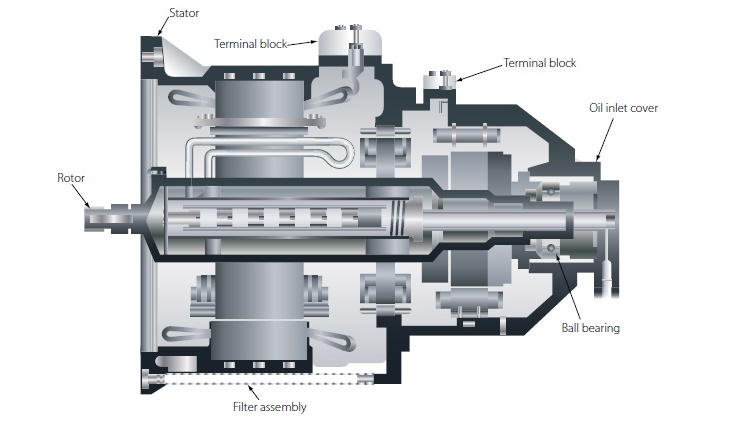
\includegraphics[width=0.9\linewidth]{img/brushless.jpg}
\caption{Vue en coube d'un alternateur sans balais}
\label{fig:brushless}
\end{figure}


On notera aussi que l'intensité du courant dans les électroaimants de l'alternateur principale peut être modifiée pour adapter le courant produit par celui-ci : un courant plus grand dans les électroaimants induira un courant produit plus grand, mais une vitesse de rotation plus faible.


\subsection{Refroidissement}
Le refroidissement des alternateurs est un problème important puisque ceux-ci tournent souvent en continu (particulièrement dans le cas des centrales nucléaires) et à de fortes charges. Le refroidissement des alternateurs se fait couramment à l'aide d'hydrogène, produit dans les centrales par électrolyse et que l'on fait circuler entre le rotor et le stator. Cet hydrogène est ensuite refroidi dans un échangeur thermique avec de l'eau.

Cette solution relativement peu onéreuse (même s'il convient alors de faire très attention à l'étanchéité de l'alternateur) permet d'obtenir de très hautes disponibilités des turbo-alternateurs.


\section{Synchronisation}
Tous les turbo-alternateurs des centrales d'un réseau électrique national (ou international) doivent fonctionner simultanément, ce qui pose des problèmes importants de synchronisation des éléments. En effet, tous ces alternateurs doivent fournir un courant de même tension, de même fréquence, en phase, et dont la somme des intensités correspond à la demande.

La fréquence est déterminée par la vitesse de rotation des turbines et le nombre de bobines sur l'alternateur. Ce nombre n'est bien sûr pas modifiable rapidement, mais il est possible d'adapter la vitesse de rotation, soit en utilisant des vannes en entrée de turbine, soit en faisant varier le courant dans les électroaimants comme détaillé dans la partie précédente. Cette possibilité d'adaptation permet à la fois de régler la phase de l'alternateur dans l'étape initiale de synchronisation, et de s'assurer que la vitesse de rotation est constante en fonctionnement malgré des variations possibles de la charge de la centrale.


\chapter{La centrale nucléaire}

\section{Principe de fonctionnement}
Un réacteur nucléaire comprend toujours au moins un cœur où se déroule la réaction de fission nucléaire, des réflecteurs et des moyens de contrôle de la réaction, une cuve métallique, et enfin une enceinte de confinement.

Les noyaux atomiques très lourds tels que l'uranium ou le plutonium contiennent énormément de protons, et sont instables. Si l'un de ces atomes très lourd (par exemple l'uranium 235 ou le plutonium 239) capture un neutron, il se transforme en un noyau encore plus instable (${}^{236}U$ ou ${}^{240}Pu$), et récupère par la même occasion de l'énergie.

Le noyau résultant se divise très rapidement: il fissionne, en se divisant en deux noyaux principaux, et en libérant deux ou trois neutrons supplémentaires, libres. Ces neutrons supplémentaires sont disponibles pour d'autres fissions de noyau : c'est le principe de la réaction en chaîne.

La différence d'énergie de liaison est partiellement transformée en énergie cinétique des produits de fission. Ceux-ci donnent cette énergie sous forme de chaleur par des chocs sur le matériau environnant. Cette chaleur est évacuée à l'aide d'un réfrigérant et peut, par exemple, être utilisée pour le chauffage ou la production d'électricité. 

Les nouveaux noyaux issus de la division sont appelés produits de fission. Ils présentent généralement un excès de neutrons, et tendent à être radioactifs avec une radioactivité $\beta^{-1}$. Quand cette radioactivité $\beta^{-1}$ a été exprimée, ils possèdent globalement une énergie de liaison plus importante par nucléon que les anciens atomes lourds — et donc sont plus stables.

Le fonctionnement est illustré figure \ref{centrale}.

\begin{figure}[h]
	\centering
	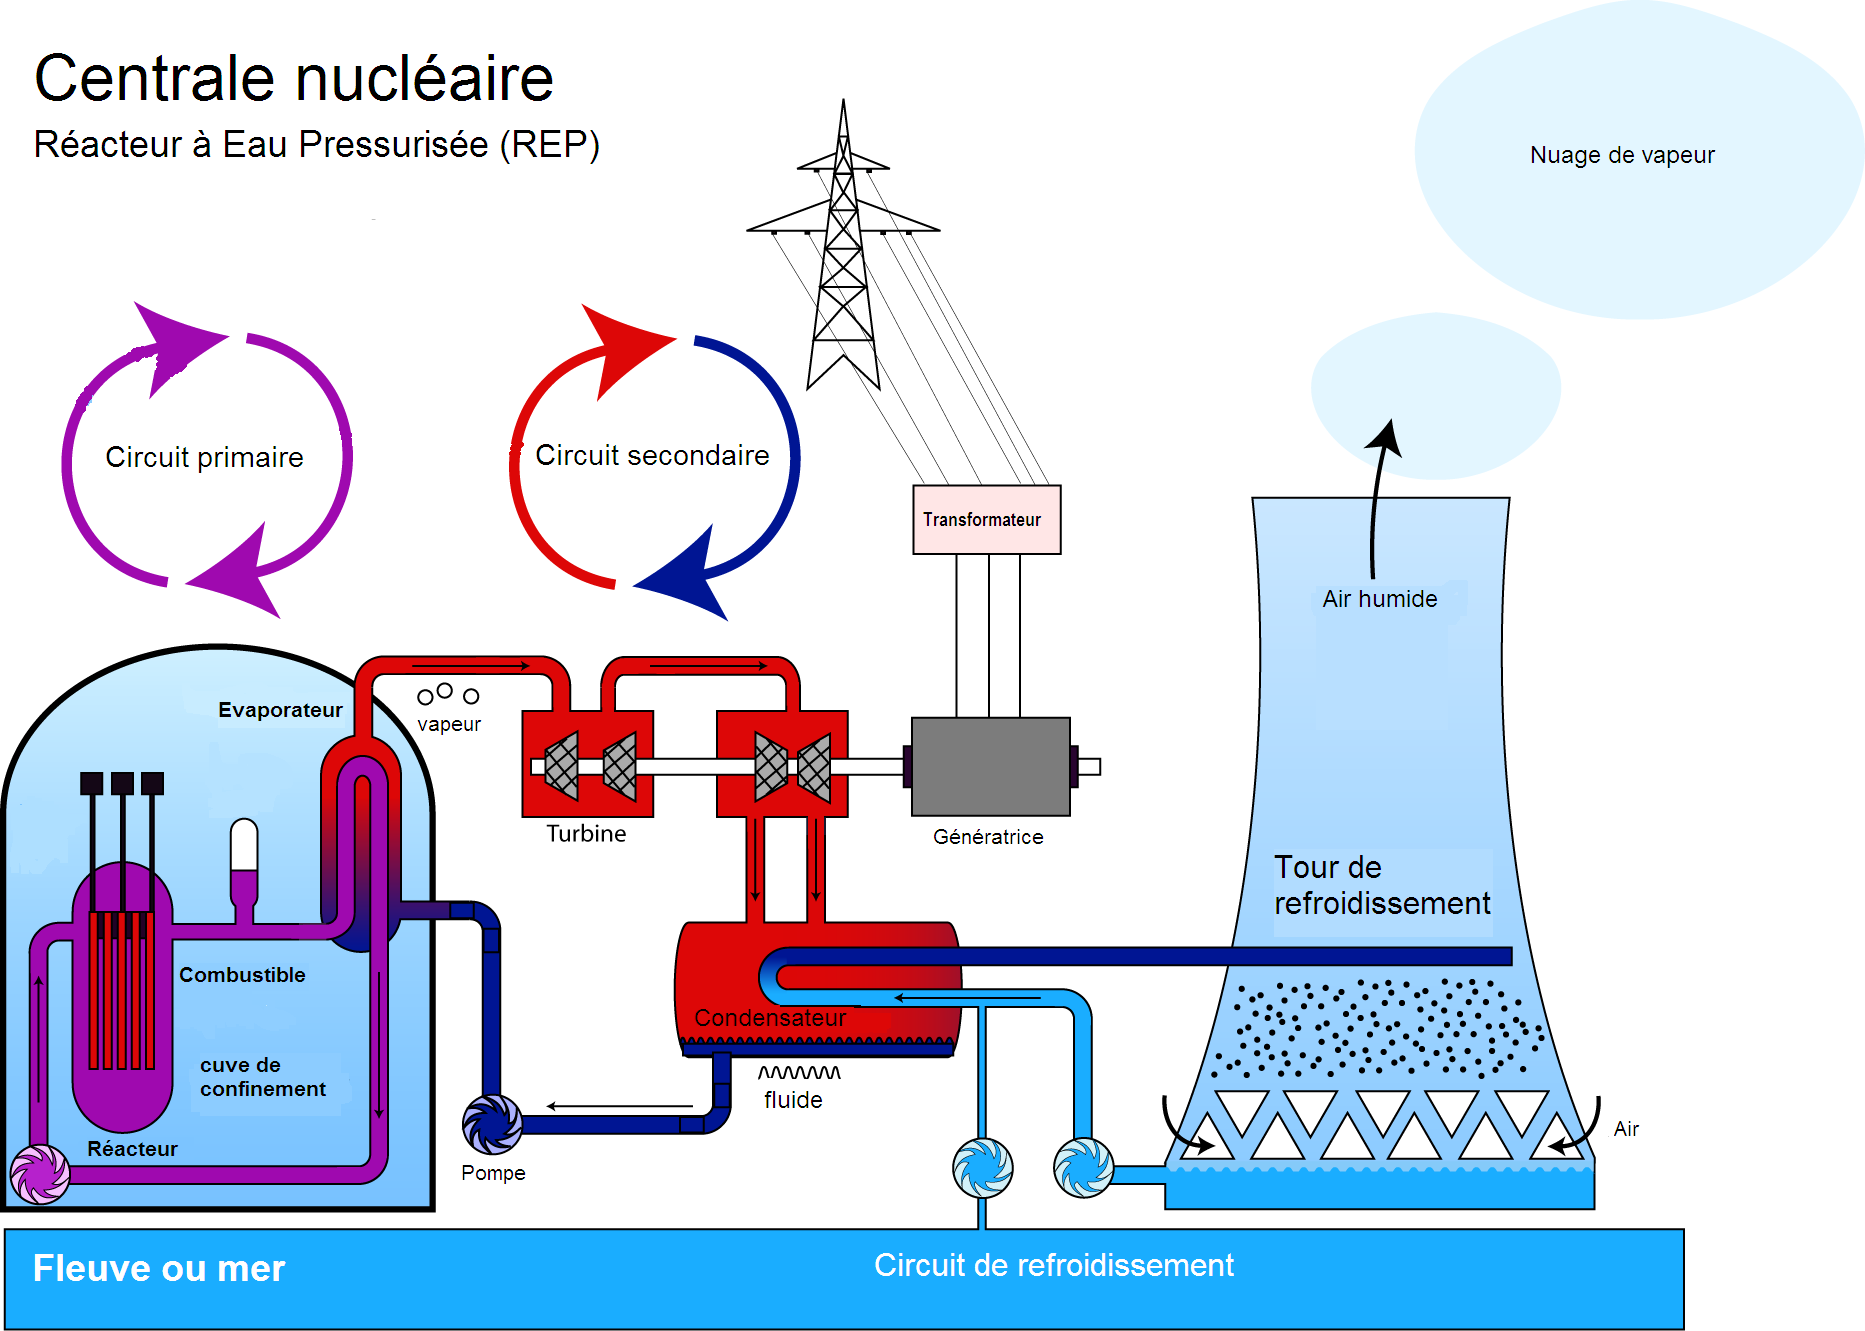
\includegraphics[width=\textwidth]{img/centrale.png}
	\caption{Schéma d'une centrale de type REP (réacteur à eau pressurisée)}
	\label{centrale}
\end{figure}

\section{Différents types de réacteurs nucléaires}
\section{Avantages et inconvénients}

\subsection{Avantages}
L'énergie nucléaire présente plusieurs avantages majeurs par rapport aux autres sources d'énergie. Une centrale nucléaire est capable de produire de l'énergie en continu pendant longtemps, et est très peu affectée par des contingences extérieures telle la météo, contrairement à la plupart des énergies renouvelables (qui dépendent du vent, de l'ensoleillement etc.).

Un autre argument en faveur de l'énergie nucléaire est son prix compétitif. En effet elles sont peu chères par rapport à d'autres sources d'énergie.

Les rejets sont pus faibles que les sources d'énergie fossiles. En effet, la fumée provenant des cheminées de centrales nucléaire est en fait de la vapeur d'eau provenant des tours de refroidissement. 

Les centrales nucléaires rejettent de la vapeur d'eau encore chaude, donc ce type de centrale est très adapté à la cogénération.


\subsection{Inconvénients}
Le premier inconvénient de l'énergie nucléaire est la production de déchets radioactifs. Ces déchets doivent être transportés puis stockées dans un lieu sur pendant longtemps.

La durée de construction d'une centrale nucléaire est de 10 ans, et sa durée de fonctionnement n'est que de 30 à 40 ans.

De plus, la production d'énergie nucléaire est difficilement adaptable à la demande d'énergie et à ses fluctuations journalières et hebdomadaires. En effet, les centrales nucléaires présentent une inertie importante en ce qui concerne la modification de la quantité d'énergie produite. Un barrage hydraulique peut, au contraire, ouvrir ou fermer les vannes en quelques minutes.

Enfin, l'emploi de matériaux instables et très énergétiques par nature rend cette forme de production d'énergie particulièrement dangereuse. Des accidents majeurs, tels Chernobyl ou plus récemment Fukushima nous rappellent les dangers de cette technologie.

\section{Implémentation}










\chapter{Le barrage hydroélectrique}

\section{Introduction et utilisation}
L'énergie hydroélectrique est une source d'énergie renouvelable et relativement propre, même si elle nécessite de gros travaux et des investissements importants.

Environ 16\% de la production mondiale d'électricité, et 13.3\% de la production française, sont dûs à l'hydroélectrique. Il y a en France 399 barrages, d'une capacité totale de \unit[25]{GW}, soit environ \unit[62]{MW} pour un barrage moyen. Avec \unit[196]{GW} de puissance installée, c'est la Chine qui a la plus grosse capacité de production hydroélectrique, devant le Canada et le Brésil. 

\section{Principes de fonctionnement}
Le terme d'énergie hydroélectrique est relativement vaste et recouvre tous les moyens de produire de l'électricité à partir des réserves d'eau. On trouve principalement deux types de centrales :
\begin{itemize}
	\item Les centrales fluviales, qui sont installés soit directement le long d'un fleuve, soit avec un barrage et un lac de retenue. Ces centrales fonctionnent toutes avec des turbo-alternateurs, en forçant l'eau qui s'écoule à passer par des turbines.
	\item Les centrales maritimes, qui peuvent utiliser l'énergie des courants marins (leur fonctionnement est alors assez similaire à celui d'éoliennes) ou celle de la marée (dans ce cas, elles fonctionnent globalement comme des barrages fluviaux).
\end{itemize}

Les barrages ont aussi souvent une finalité de contrôle des crues ou du débit des rivières.

\begin{figure}[h]
	\centering\hspace*{-5mm}
	\begin{minipage}{.5\textwidth}
		\centering
		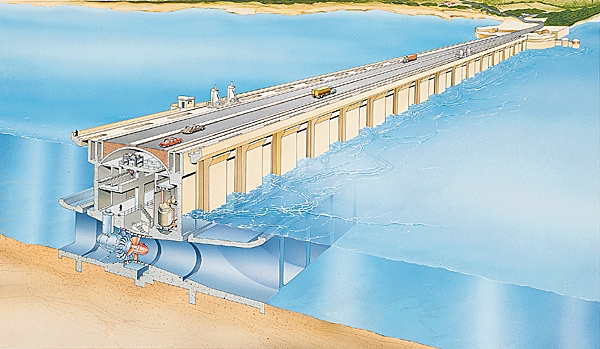
\includegraphics[width=\linewidth]{img/maremotrice}
		\caption{Une centrale hydroélectrique marémotrice}
		\label{fig:maremotrice}
	\end{minipage}%
	\hspace*{1cm}
	\begin{minipage}{.5\textwidth}
		\centering
		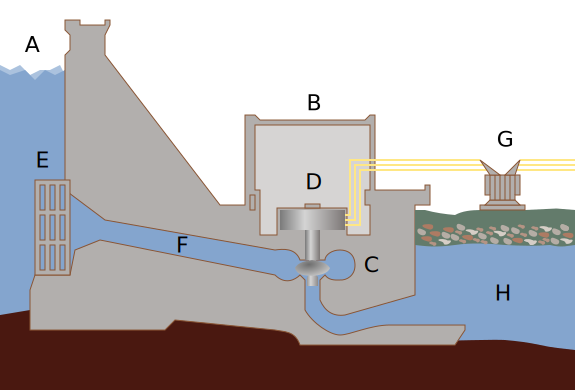
\includegraphics[width=\linewidth]{img/barrage_coupe}
		\caption{Coupe d'un barrage hydroélectrique}
		\label{fig:barrage_coupe}
	\end{minipage}
\end{figure}

\section{Avantages et inconvénients}
L'énergie hydroélectrique, sous toutes ses formes, a l'avantage d'être renouvelable -- elle utilise en fait indirectement l'énergie solaire qui fait s'évaporer l'eau terrestre, pour les barrages, ou le vent qui crée les vagues.

Malgré des coûts de réalisation généralement élevés, les coûts de maintenance sont raisonnables et les installations relativement durables. En revanche, ils doivent de plus être placés dans des zones montagneuses appropriées, qui sont en nombre limité et peuvent être très rares dans certaines parties du monde\textellipsis

Les risques en cas de problèmes structurels sur les barrages hydroélectriques sont très importants : on rappellera par exemple l'accident de Malpasset, en France, où l'écroulement d'un barrage a fait plus de 400 victimes et des dégâts matériels impressionnants (figure \ref{fig:malpasset}). L'exemple du barrage des Trois-Gorges, en Chine, montre aussi les dégâts écologiques qui peuvent être causés par des travaux de barrage, notamment par l'inondation de forêts, le blocage des sédiments, et le blocage des migrations de poissons (bien qu'il soit de plus en plus fréquent d'installer des passages pour saumons dans les barrages).

\begin{figure}
\centering
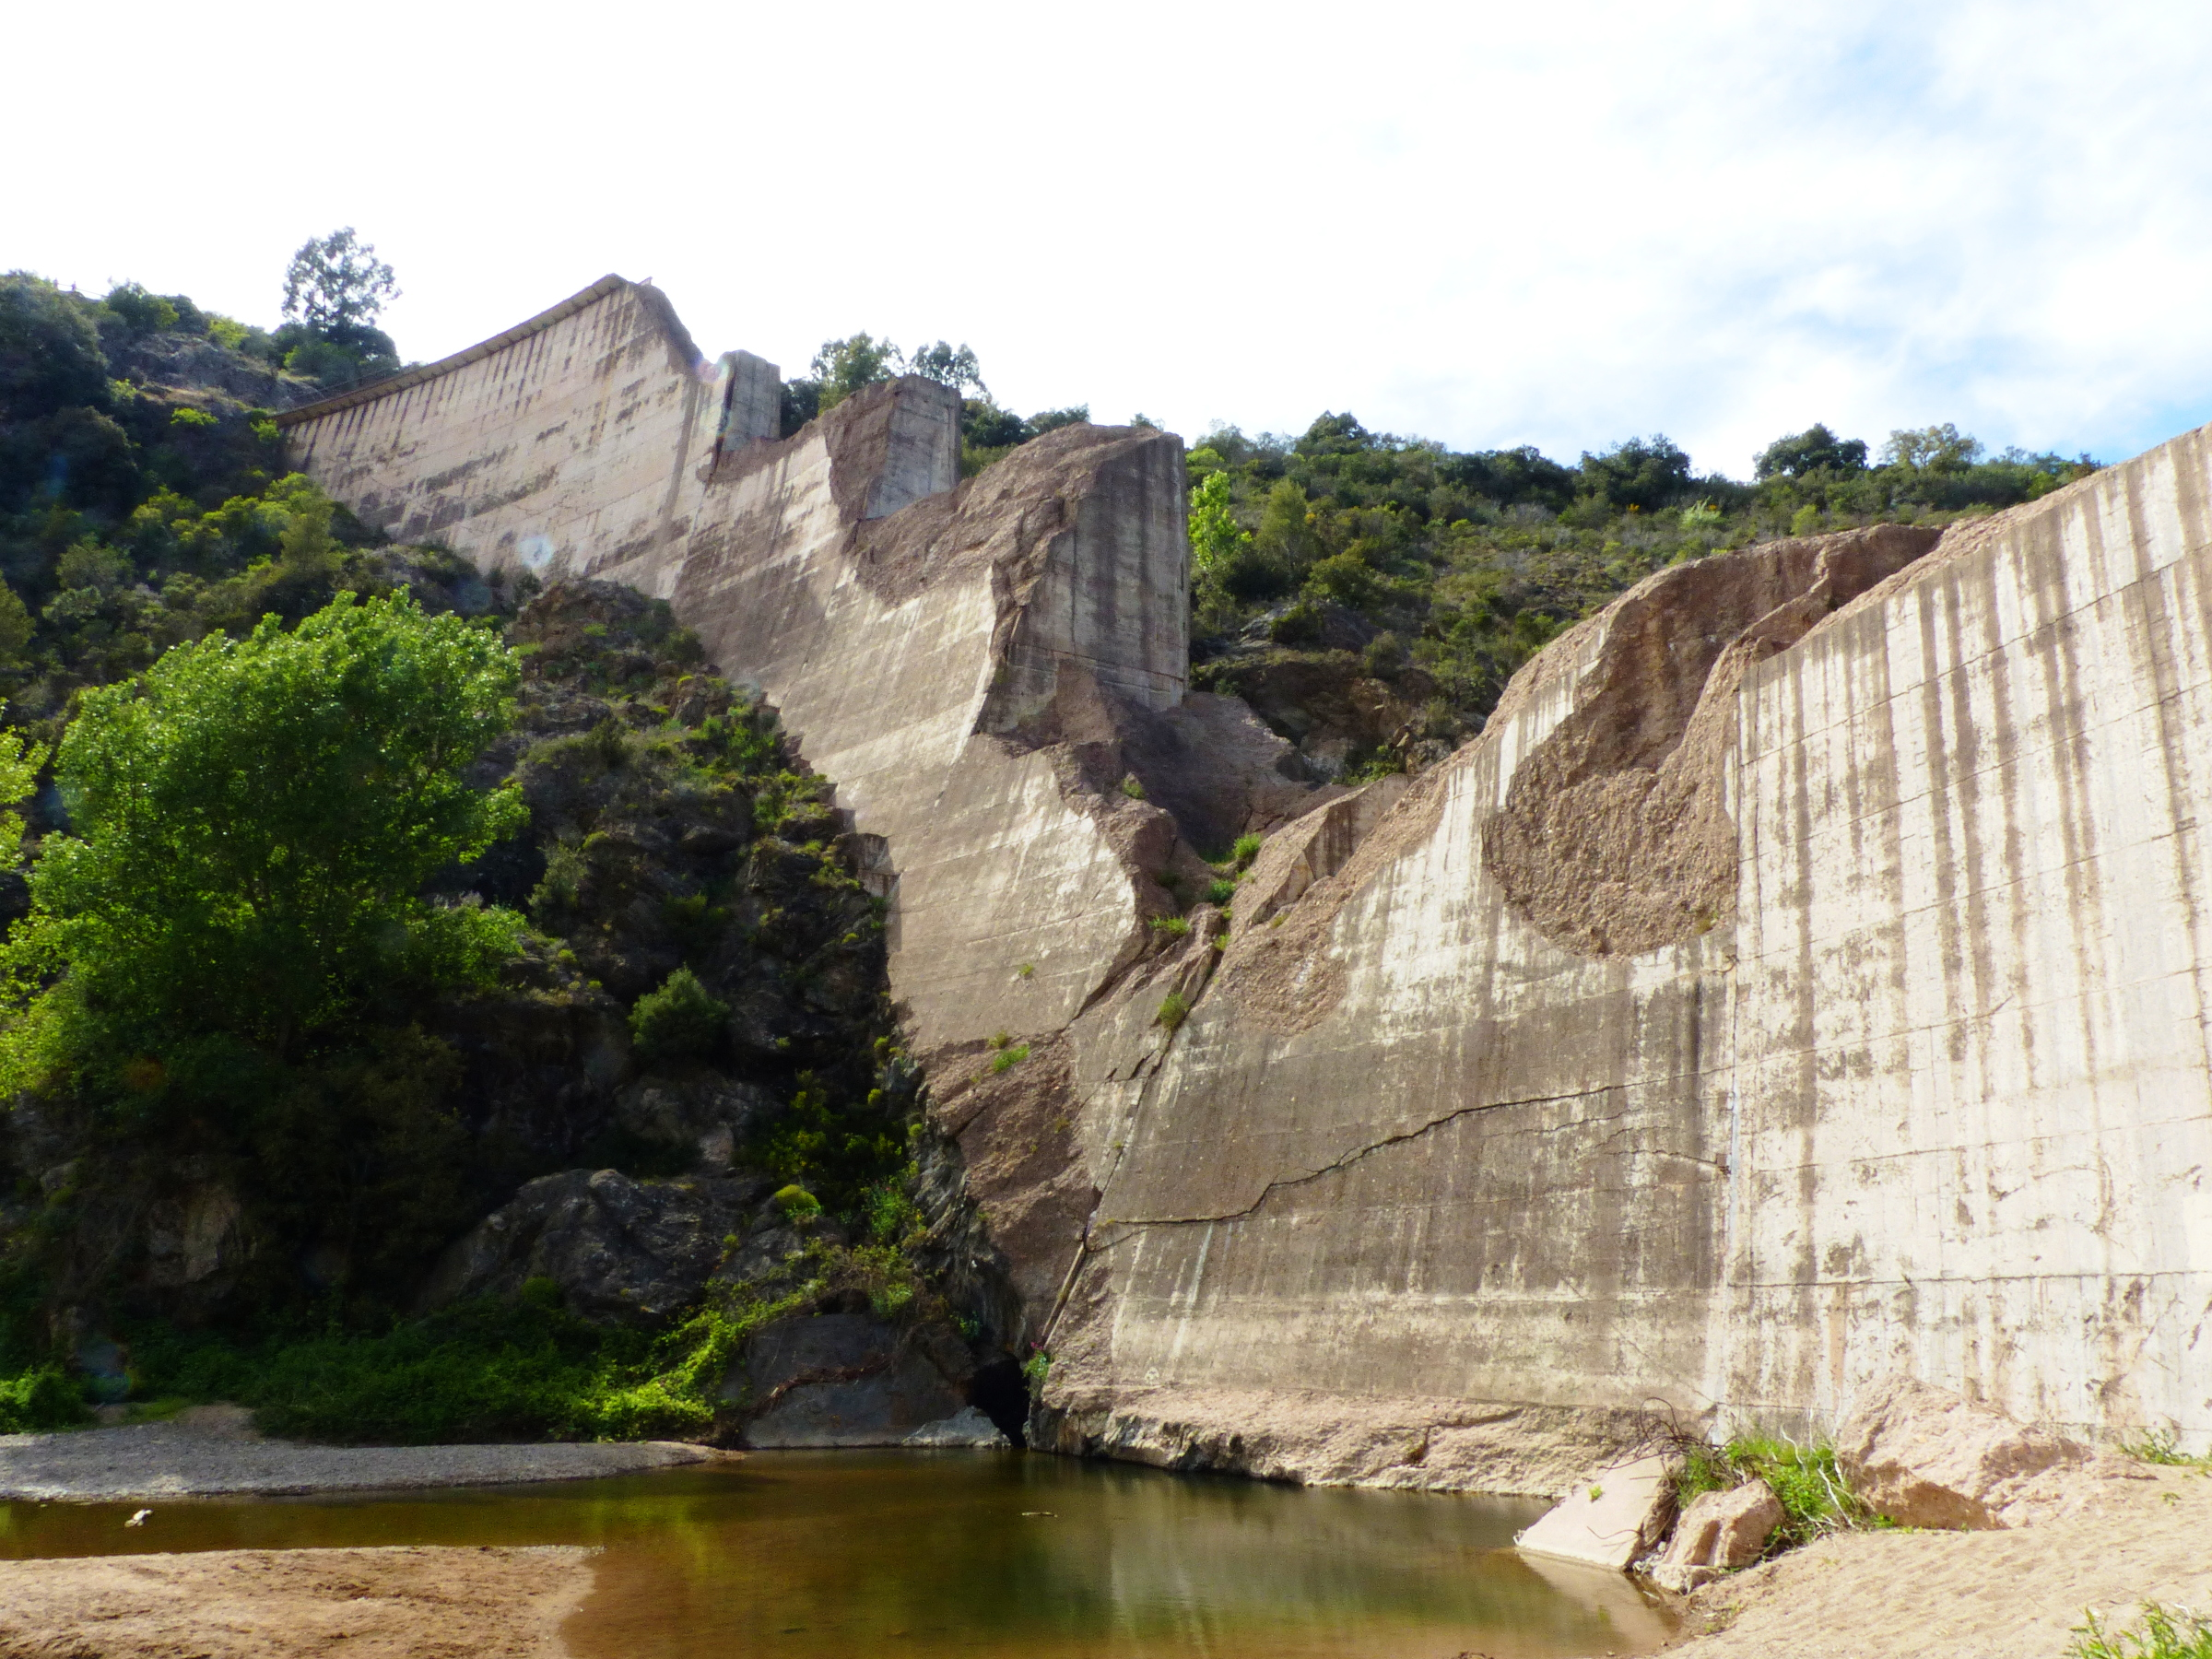
\includegraphics[width=0.9\linewidth]{img/malpasset.jpg}
\caption{Les restes du barrage de Malpasset}
\label{fig:malpasset}
\end{figure}

Un avantage bien connu des barrages hydroélectriques est aussi celui du stockage de l'énergie par pompages. De nombreuses centrales sont capables d'inverser le fonctionnement de leurs turbo-alternateurs pour pomper l'eau dans le lac de retenue. Le rendement d'une telle opération est d'environ 70 à 80\%. Ceci permet notamment de combler certains inconvénients des sources de production peu adaptables, comme les centrales nucléaires, ou dont la production est difficile à contrôler, comme les éoliennes ou le photovoltaïque.

Les barrages disposent dans tous les cas d'une réactivité énorme puisqu'il suffit d'ouvrir ou de fermer les vannes de la retenue pour arriver à la production maximale ou au contraire l'arrêter totalement. Les centrales marémotrices n'ont pas cette faculté mais ont toutefois l'avantage d'être extrêmement régulières, encore une fois au contraire de la majorité des autres sources d'énergie renouvelables.

\nocite{*}
\printbibliography
\end{document}
